\section{System Modeling}
\phantomsection

% TODO refactor diagram captions

This chapter contains an attempt to model the application by use of UML
diagrams so that the further development of the system is easier and has well
defined boundaries. As a rule, the process of modeling an information system
usually starts off by laying out a general picture and then deepens into more
detailed views of the inner workings of the system.


\subsection{Use Case Layout of the Game}

Use case diagrams are used to provide a good understanding of what a user can
do with the application in question. In a nutshell, a game is out there to be
played and the 'Snowfight' is no exception. The gameplay has a rather simple
concept behind it and includes several things:

\begin{itemize}
	\item Moving around the field
	\item Throwing snowballs at adversaries
	\item Being eliminated from a game by being hit with snowballs
	\item Using the phone as a controller device
\end{itemize}

Besides playing the game itself, the players are able to view game results after
a match has finished and they can also modify the character's appearance and
name before the game starts.

\begin{figure}[!h]
\centering
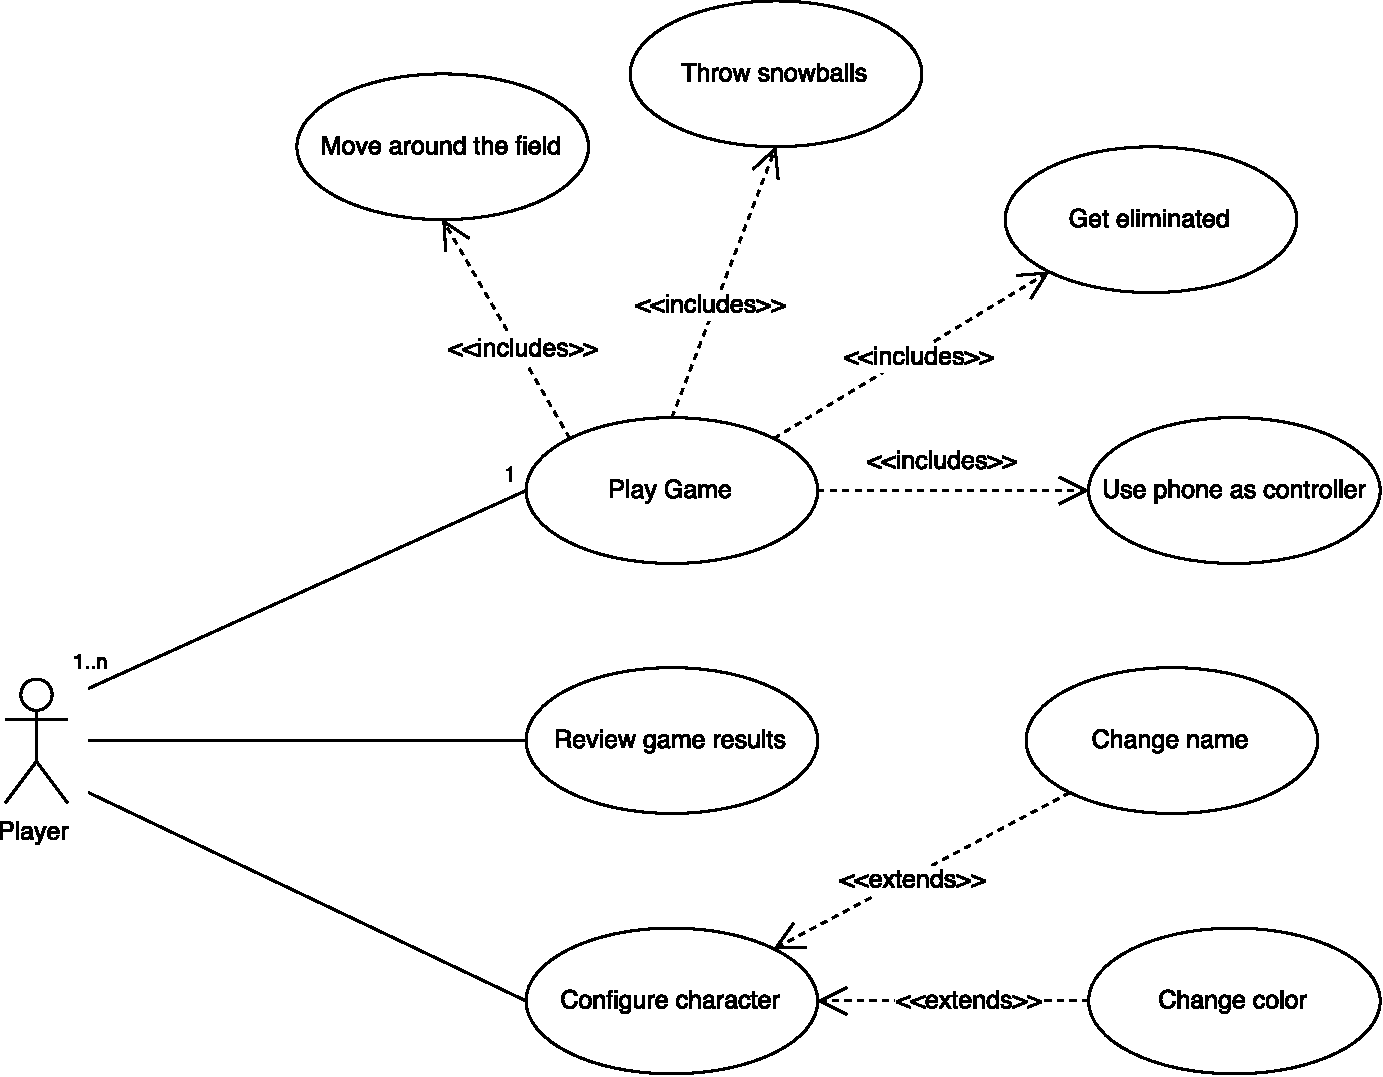
\includegraphics[width=15cm]{diagrams/usecase}
\caption{Game Use Cases from the Player's Perspective}\label{diag:usecase}
\end{figure}

\newpage

\subsection{User Activity Graph}

When it comes to the sequence of activities that may take place as part of the
use of an application, the activity diagram does an excellent job at
illustrating the transitions between different activities and various conditions
that might alter the activity flow.

A typical set of activities that take place as part of playing 'Snowfight' is
represented in the graph below. The players start off by accessing the index
page of the game in a web browser. This brings them in a game lobby that
contains a shareable URL used to connect controllers. Players navigate to this
URL in the browser on their smart-phones, personalize some character
configurations and connect to the game by pressing the start button on their
'controllers'. When all players are connected, the game is ready to start, which
is done by hitting the respective button in the game lobby. Now the players
enter the game loop, that is, they play a match, review the results and are
given the opportunity to restart the match and when all players make their
decisions the game is restarting leaving out those players who chose to quit.

\begin{figure}[!h]
\centering
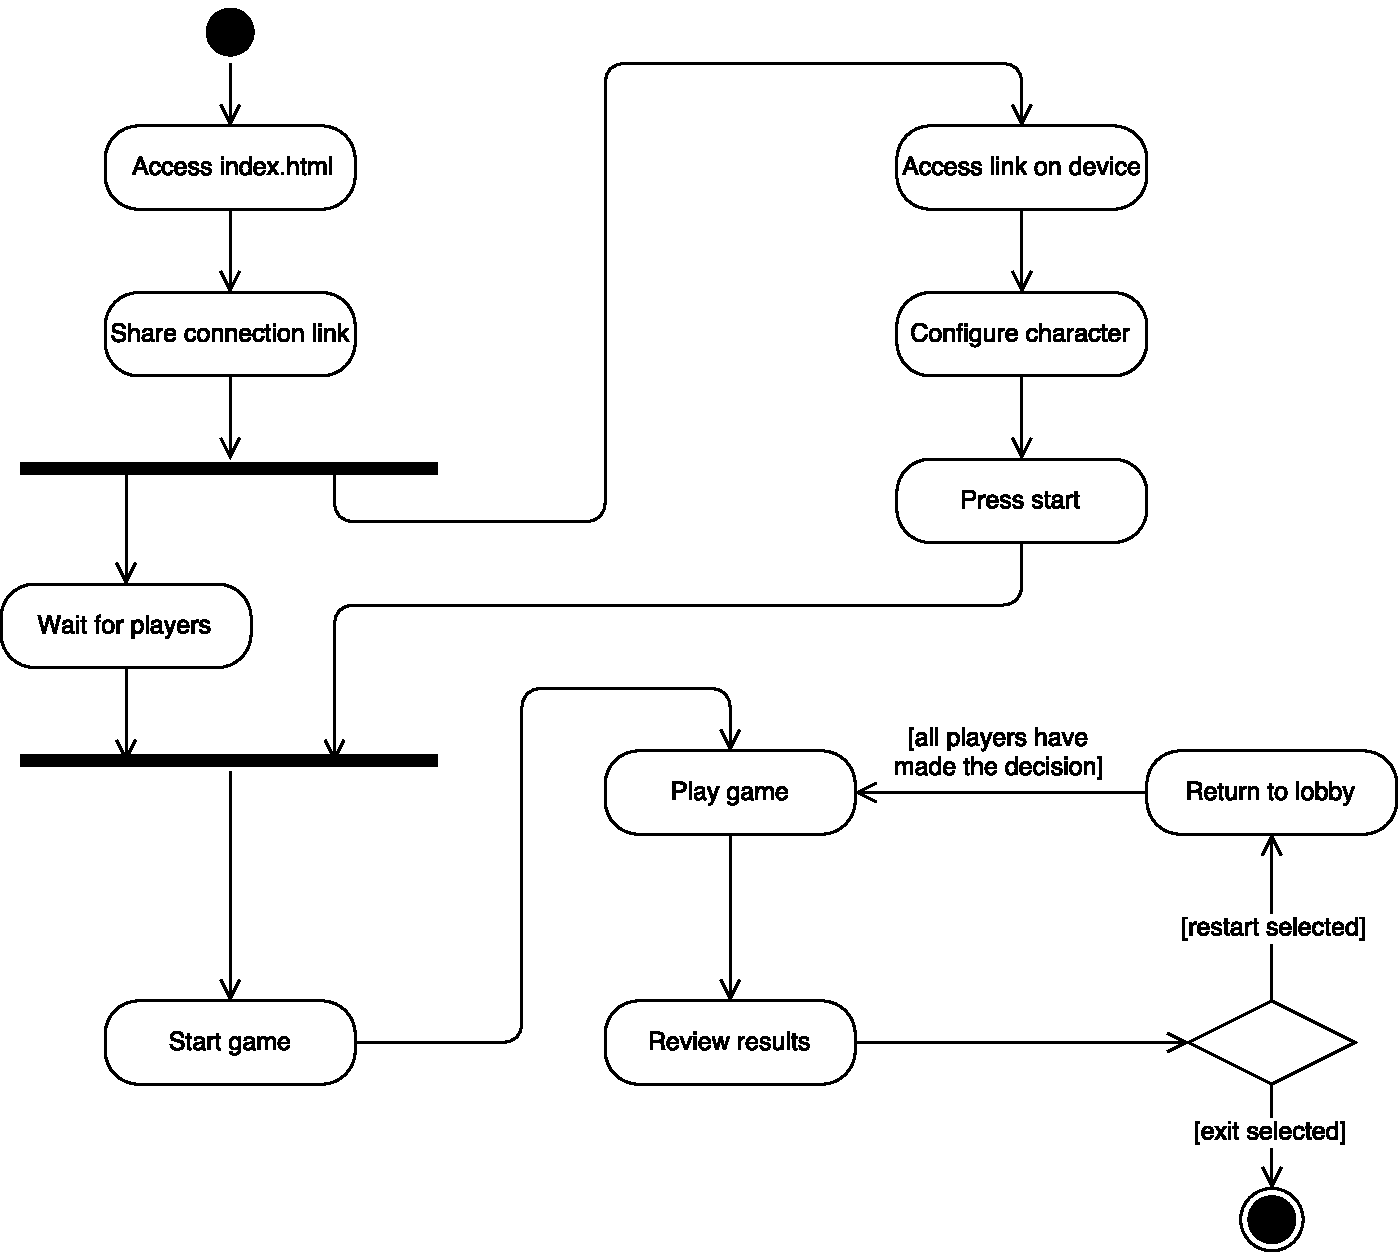
\includegraphics[width=15cm]{diagrams/activity}
\caption{Top-level Activities of the User}\label{diag:activity}
\end{figure}

\newpage

\subsection{High-level Game States}

When compared to simple web applications, games have a very substantial
distinction in the sense that they are real-time system. A web page can be
considered pretty much static once it has rendered, and all that happens
afterwards is the result of various event handlers modifying the obtained
document. Games, on the other hand, are being rendered to the screen every
fraction of a second and keep changing as a living system. All this takes place
in a, so called, game loop, and it is quite difficult to implement the various
stages the game passes through in a single chain of 'if's. This is why even at
the modeling stage, the game is split in different states through which it can
pass and which have different things to render and process.

The game in question has four main states:

\begin{description}
	\item [Lobby] - works like a simple web page and is used to gather players before game
	\item [Asset pre-loading] - is the period after the 'start' button was hit, but before the game simulation begins, and it is responsible for preparing all the assets before they are used
	\item [Active game] - the state in which the main gameplay takes place that performs all physics computations and rendering, it also includes the game logic
	\item [Results overview] - is like an interlude between matches, when the game simulation is stopped and only information about the match is rendered to the screen
\end{description}

\begin{figure}[!h]
\centering
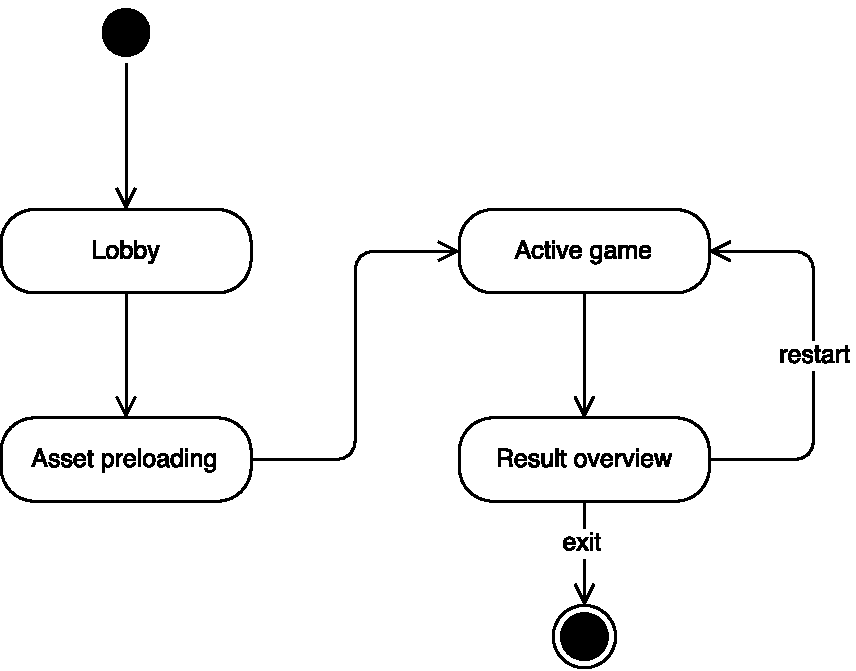
\includegraphics[width=15cm]{diagrams/state_2}
\caption{Game States}\label{diag:state_2}
\end{figure}

\newpage

\subsection{Player State Machine}

At a lower level the game logic is controlled by the states of individual game
objects and the main game object of the 'Snowfight' game is the player. It quite
convenient to model the player as a state machine because the way it is render,
the way it is updated and the manner in which it reacts to input heavily depend
on its current state. When put in real context, it becomes clear that it is not
possible to use the same animation or texture for a player that moves as well as
for a player that is disabled. In these two states the player also has different
kind of response to user input. When in default state, the player can move
around the field as a reaction to the motion controller, as opposed to the
situation of a disabled player when any kind of input has a null result.

\begin{figure}[!h]
\centering
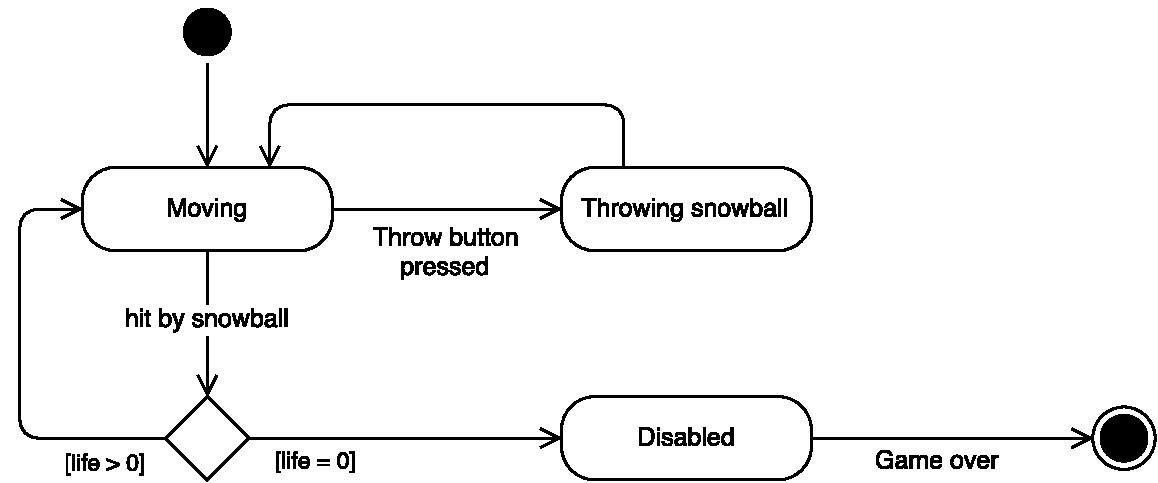
\includegraphics[width=\textwidth]{diagrams/state_1}
\caption{Player States}\label{diag:state_1}
\end{figure}

As it can be observed in the diagram above, the \emph{moving} state is the
default state as well as the first one in which the player starts the game. The
transition to another state might happen it two cases, and specifically, if the
user hits the button for throwing snowballs, the player transitions to the
respective state, the appropriate animation is played and the logic of trowing a
snowball is triggered. As soon as the \emph{throwing} process gets to its end,
the player transitions back to the \emph{moving} state automatically. In the
second case, the state change is set off by a game event rather than through
direct user input, that is, when a player is hit by a snowball of an adversary,
the state machine reaches a decision point. The amount of 'health points' of the
player in question is assessed and recalculated and if it is equal to zero, the
player enters the \emph{disabled} state and is considered eliminated from the
game till the end of the match, otherwise, an automatic transition back to the
\emph{moving} state takes place.

\newpage

\subsection{Class Hierarchy of Game Objects}

\begin{figure}[!h]
\centering
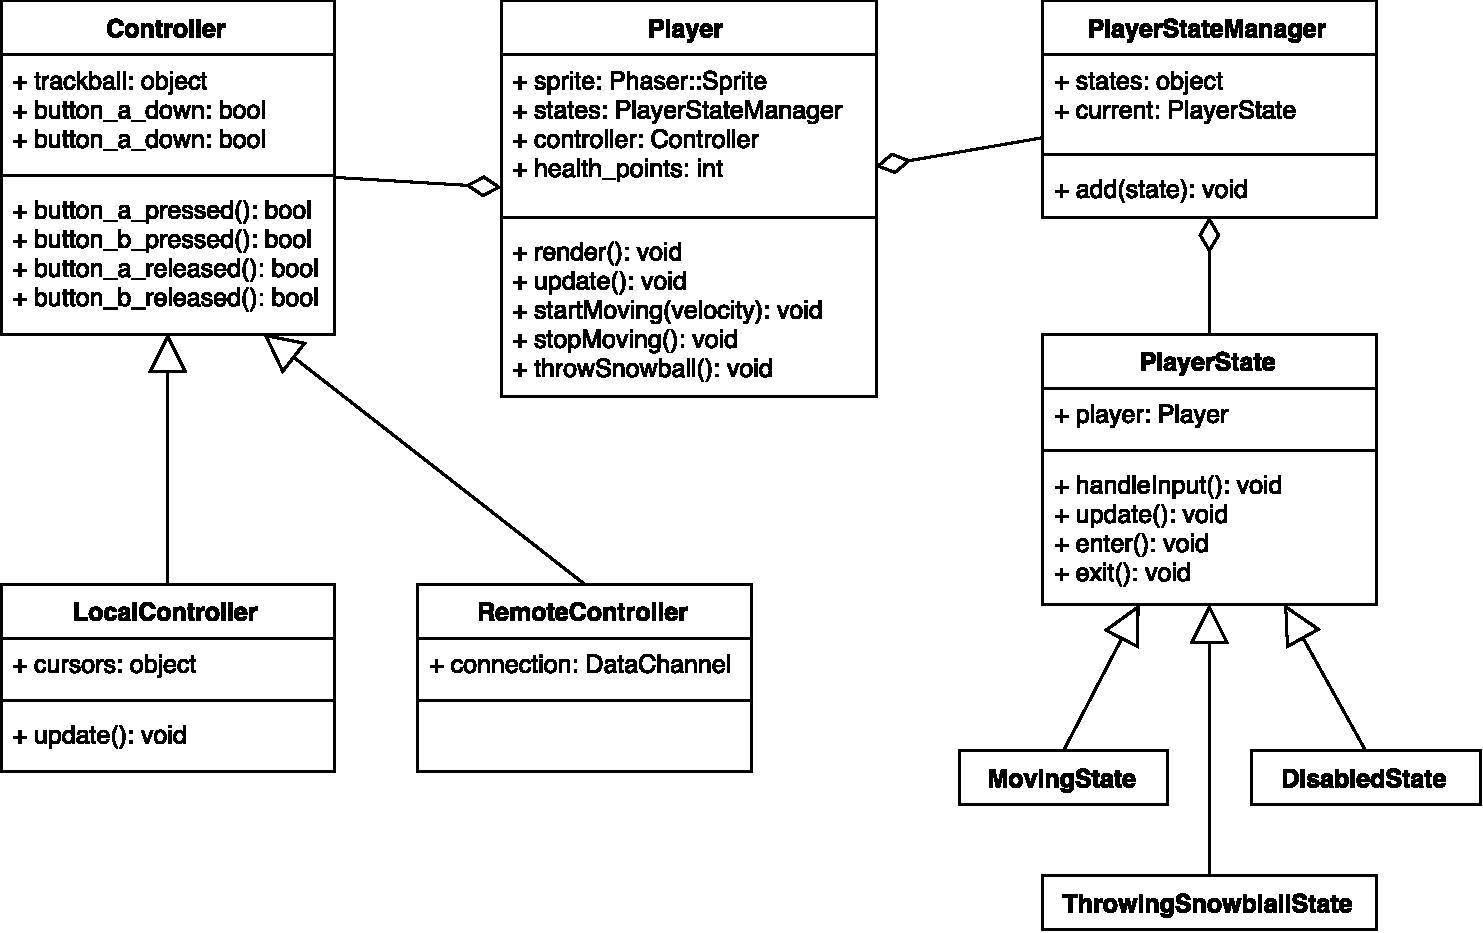
\includegraphics[width=15cm]{diagrams/class}
\caption{Class Diagram}\label{diag:class}
\end{figure}


\subsection{Components and Libraries}

\begin{figure}[!h]
\centering
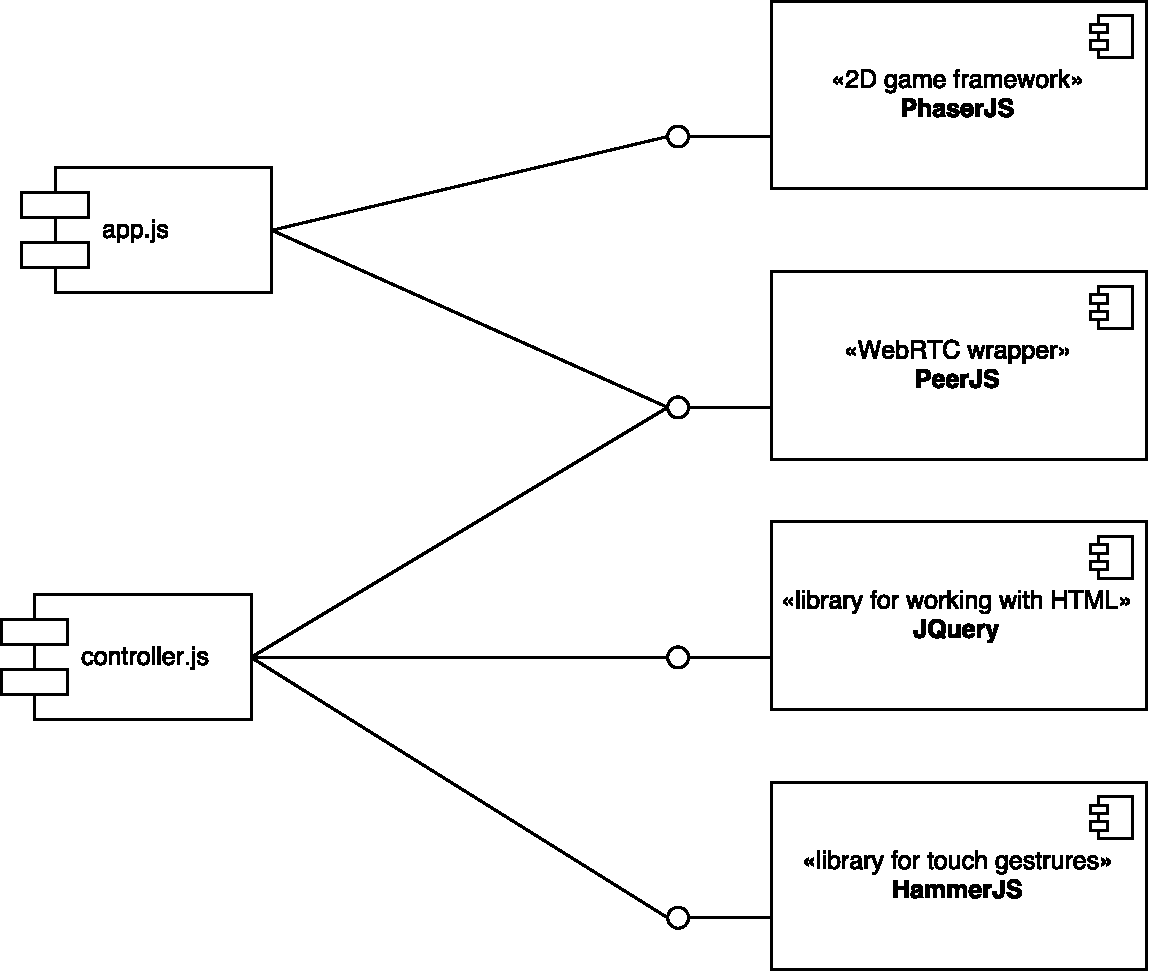
\includegraphics[width=15cm]{diagrams/component}
\caption{Component Diagram}\label{diag:component}
\end{figure}


\subsection{Deployment Setup}

\begin{figure}[!h]
\centering
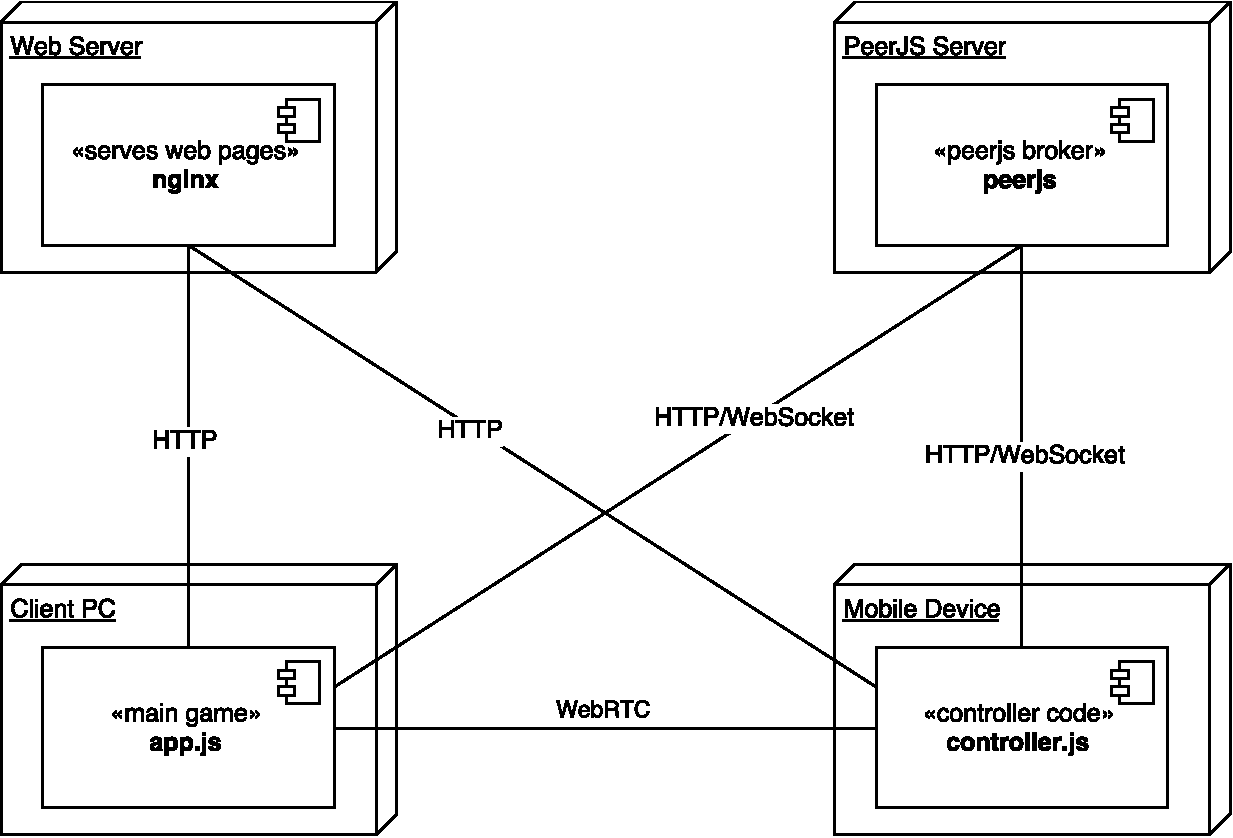
\includegraphics[width=15cm]{diagrams/deployment}
\caption{Deployment Diagram}\label{diag:deployment}
\end{figure}


\subsection{System Design Conclusions}

\clearpage
